\chapter{基于弱标签的语义分割}
% 在本文中,我们提出了一种新的三维物体分割的弱监督学习策略,以解决上述的挑战。我们的主要想法包括两个方面。首先,我们提出了一种自学习方法,通过物体样本增强的方法,来捕捉目标物体类别的三维形状先验。随后,我们将这种学习到的形状先验纳入具有形状感知的分割网络的训练过程。另外,我们采用了一个稀疏的弱标注方案,以更好地利用物体掩膜的空间连续性,并在不增加整体标注成本的情况下促进形状上下文的学习。
%为了实现这一目标,我们设计了一个由两个主要模块组成的深度神经网络:一个是标准的语义分割网络,它从三维输入图像中产生一个初始的三维分割掩膜;另一个是形状去噪网络,它对初始分割掩膜进行改进并输出一个最终的三维分割。为了训练深度网络,我们首先引入一种稀疏的弱标注方案,在该方案中,我们只标注三维数据的一个特定的二维图像切片的子集(可以将三维图像数据视作一系列连续的二维图像切片),同时对每张二维图像,我们设计了一种混合式弱标签,它结合了前景涂鸦和目标物体的一个宽松边界框。给定这样的弱标注形式,我们为前述的网络模型设计了一个迭代学习框架,交替进行像素级标签生成和网络参数更新。

在本章,我们为基于弱标签的语义分割提出一种新的结合形状先验的学习策略。我们的目标是利用物体的形状先验设计更有效的弱监督分割框架,并将其纳入训练过程。为此,我们探索自学习方法,从仅有弱标签的训练数据中学到目标类别的形状先验。更进一步,我们对比了不同的弱标注策略,并提出一种新的混合式标注方法,来为弱监督学习提供更有效的训练信息和更好的性能。我们采用了迭代学习的方法,来逐步地提升分割效果,直至模型参数收敛。

% 各小节介绍
本章分为以下五个部分。在第一节我们对基于弱标签的语义分割任务进行介绍,第二节介绍我们提出的结合形状先验的弱监督分割模型。然后,在第三节我们提出新的高效的稀疏弱标注策略,随后在第四节详细介绍了模型的训练方法,特别是自学习形状模型的策略。第五节为实验部分,包括实验设置、实验细节、定量结果、定性结果、消融实验等。最后一节是本章总结。

\section{问题概述}
医学图像的分割任务如图~\ref{c3_fig1}所示,左侧为二维图像及其分割结果,右侧为三维图像及其三维分割可视化(三维图像由一系列连续的二维图像堆叠成统一的整体)。
特别地是,基于弱标签的语义分割,其训练样本采用了弱标签而非全标签的形式。
给定一个输入的三维体积图像 $\mathbf{I} \in \mathbb{R}^{H \times W \times D}$,我们的目标是估计其分割掩膜 $\mathbf{M} \in \mathcal{S}^{H \times W \times D}$,其中 $H$ and $W$ 是图像切片的高度和宽度,$D$ 则是组成三维图像的切片数目。$\mathcal{S} = \{0, 1\}$ 是语义标签集,其中 $0$ 表示背景类,$1$ 为前景类。
训练数据集 $\mathcal{D} = \{\mathbf{I}^n, \mathbf{Y}^n\}_{n=1}^N$,其中 $\mathbf{Y}^n \in \mathcal{S}'^{H \times W \times D}$ 是 $\mathbf{I}^n$ 对应的弱标签, $\mathcal{S}' = \mathcal{S} \cup \{u\}$ 且 $u$ 代表无标签像素,$N$ 是训练数据样本的数目。
在本文中,我们关注二分类分割问题,即只有前景类别和背景类别。我们的方法可以通过单独处理每个类别来应用在多分类问题。

这个工作中我们的核心思想是,从弱标签中得到一个自学习的形状先验,然后利用这个形状先验来进一步进行形状去噪和改进。为了实现这一目标,我们设计了一个由两个主要模块组成的深度神经网络:一个语义分割模块和一个形状去噪模块。我们首先用语义分割模块在输入图像上预测一个初始的粗分割掩膜,然后形状去噪模块在初始掩膜上应用自学习的形状先验来进行去噪和改进。为了进一步利用形状先验来改进模型,我们采用了一种迭代学习框架,它在生成伪标签和更新模型参数之间迭代进行。我们的模型概览见图~\ref{fig:model}。


    \begin{figure*}[tbp]
        \centering 
        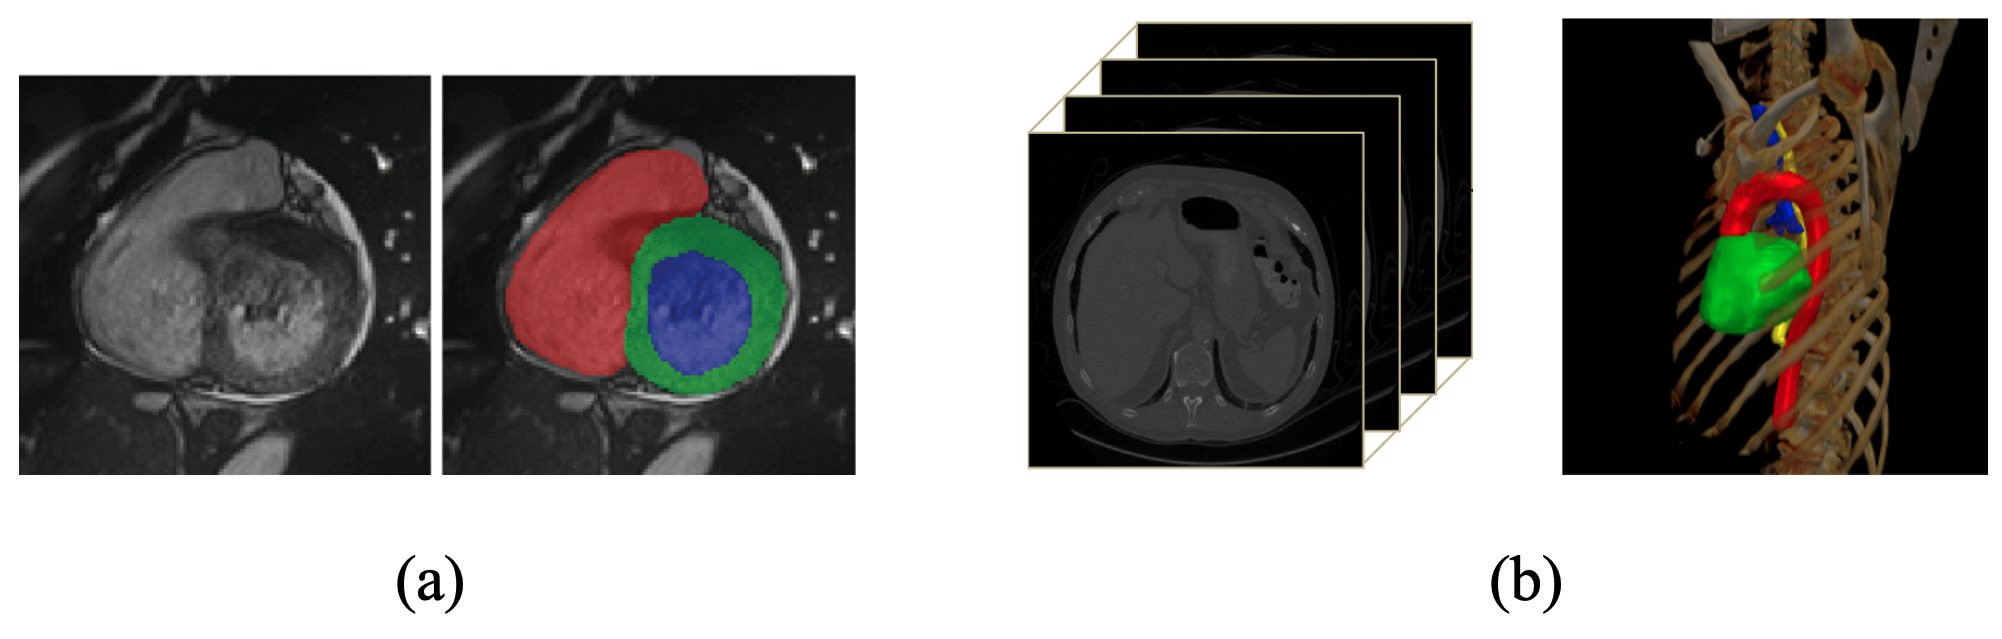
\includegraphics[width=1.0\textwidth]{img/c3/c3_1.png}
        \bicaption{医学图像的语义分割任务示例。左侧为二维图像与分割标签,右侧为三维图像(由一系列连续的二维图像组成)及其标签。}
        {Examples of medical image semantic segmentation. (a) 2D image and its segmentation label. (b) 3D image and its segmentation label.}
        \label{c3_fig1}
    \end{figure*}

    \begin{figure*}[t!]
        \centering 
        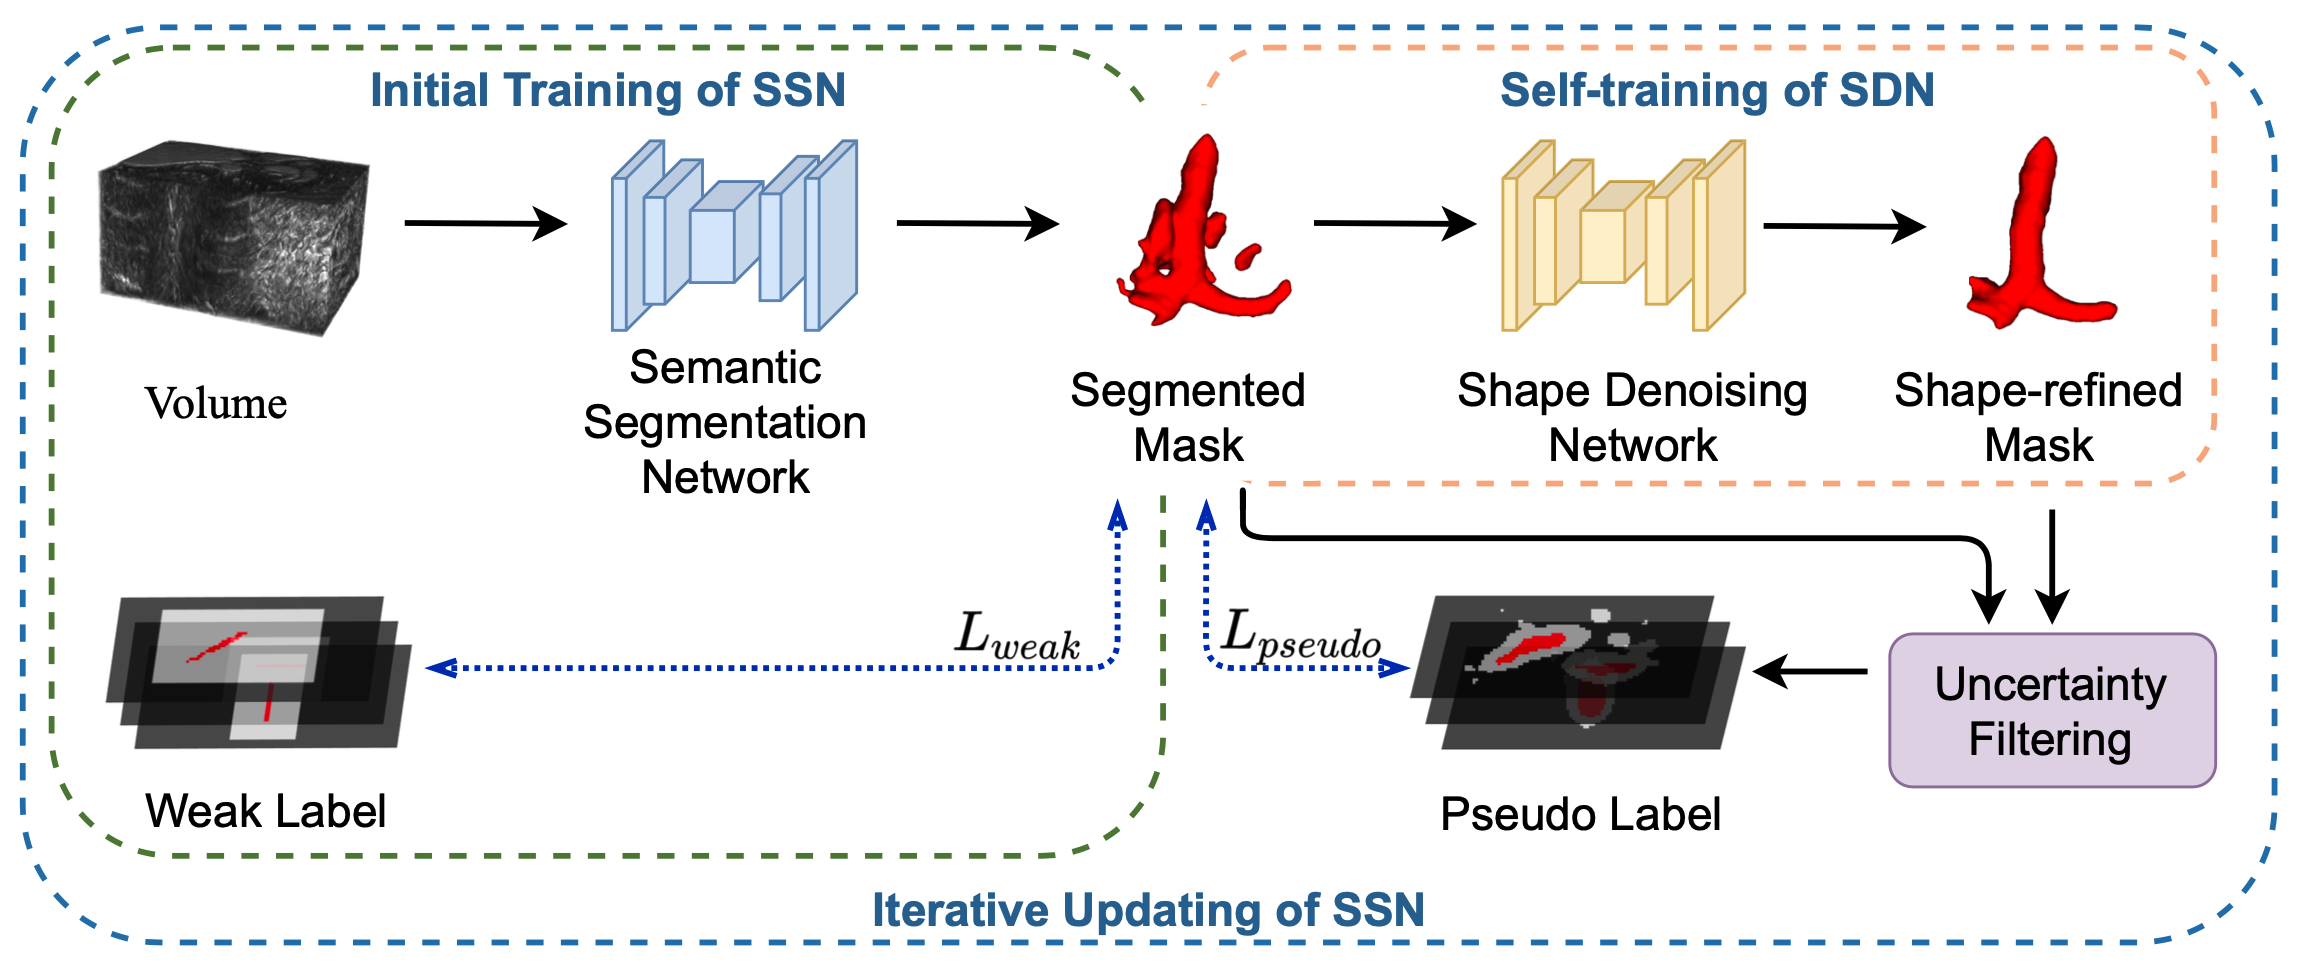
\includegraphics[width=1.00\textwidth]{img/c3/b_model_shape.png}
        \bicaption{弱监督语义分割模型概览。我们的模型由两个主要模块组成:语义分割网络和形状去噪网络。语义分割网络从输入的体积图像中预测出一个初始的分割掩膜,并由其后形状去噪网络进一步完善,作为最终输出。我们采用一种迭代训练的方法来训练模型。}
        {The overview of our method. Our model consists of two main modules: Semantic Segmentation Network (SSN) and Shape Denoising Network (SDN). Our SSN predicts an initial segmented mask from the input volumetric image, which is further refined by our SDN as final output. To train our model, we propose an iteraitve learning strategy.}
        \label{fig:model}
    \end{figure*}


\section{模型设计}
在本节我们详细介绍模型中的两个主要模块:语义分割网络和形状去噪网络。

\textbf{语义分割网络} 语义分割网络 $\mathcal{F}_{SSN}$ 用来产生一个初始的粗分割掩膜,它将一个体积图像 $\mathbf{I}$ 作为输入,并输出一个概率图 $\mathbf{P}_s \in [0,1]^{H\times W\times D}$,表示每个像素属于前景的置信度。由 $\mathbf{P}_s$ 我们可以得出初始的前景分割掩膜 $\mathbf{M}_s$:$\mathbf{P}_s = \mathcal{F}_{SSN} (\mathbf{I}; \Theta), \mathbf{M}_s = \mathds{1} (\mathbf{P}_s > 0.5)$,其中 $\Theta$ 表示 $\mathcal{F}_{SSN}$ 的参数,而 $\mathds{1}(\cdot)$ 是一个指示函数。
我们用 nnU-Net~\citep{isensee2019automated} 来实例化我们的语义分割网络,它是医学图像语义分割的最先进而广泛的模型结构。
% 可扩展:将 模型的具体设计可再讲一段,从附录 C 里取出。


\textbf{形状去噪网络} 我们设计了一个形状去噪网络 $\mathcal{F}_{SDN}$ 来编码一个统一的形状先验,然后应用于初始的粗分割掩膜上进行形状改进。形状去噪网络的思想借鉴自去噪自编码器\citep{vincent2010stacked}和增强自编码器\citep{Sundermeyer_2018_ECCV}。去噪自编码器将图像编码为对噪声不敏感的隐向量,以表示原始的干净图像。增强自编码器产生输入图像中物体的方向编码,而对其他变换和环境条件具有不变性。与这些旨在为图像或物体方向提供代表性向量表征的方法不同,我们的目标是将输入的粗分割掩膜中恢复为干净而完整的形状。
给定语义分割网络输出的初始掩膜 $\mathbf{M}_s$,我们的形状去噪网络隐式地施加了自学习的形状先验约束,并输出一个干净的形状改进的分割掩膜:$\mathbf{P}_d = \mathcal{F}_{SDN} (\mathbf{M}_s; \Omega), \mathbf{M}_d = \mathds{1} (\mathbf{P}_d > 0.5)$,其中 $\Omega$ 表示 $\mathcal{F}_{SDN}$ 的参数。由于我们的输出目标是最终的分割掩膜,而不是隐向量表示,我们的 $\mathcal{F}_{SDN}$ 采用了与 $\mathcal{F}_{SSN}$ 相同的 U-Net 结构,这种设计使得形状去噪网络在中间瓶颈层也保持较大的空间分辨率,并包含跳跃连接以捕捉更多的分割细节。

\section{弱标注策略}



\section{模型训练}



\section{实验}


\subsection{实验设置}




\subsection{实现细节}




\subsection{定量结果}




\subsection{定性结果}




\subsection{消融实验}



\section{实验}
